
\chapter{Background and Literature Review}
\label{Chap:Background}

\section{Introduction}

This chapter critically analyses literature related to the background of the research area and the data mining and analysis methods subsequently deployed with the proposed temporal rule-based classification method. This chapter thus covers the topics of traditional and temporal classification and assessment measures.

As this thesis also proposes a method for calculating changes over time using clustering and \acrfull{cvi}, So that the used clustering methods and their features are discussed in this chapter along with different types of internal and external cluster validity indices.

Multiple real-world data sets are used in this thesis as case studies derived from a public goods game and stock market data. Thus these topics are also briefly covered in this chapter.

The literature and topics in this chapter are ordered according to their importance and closeness to the proposed methods.


\section{Machine Learning and Pattern Recognition}

Pattern recognition is a branch of computer science concerned with the methods of finding patterns in raw data automatically using computer algorithms. Due to the complexity of the patterns and irregularities that can be found among the same group of patterns, it is not trivial to hard code a machine to find all patterns with acceptable accuracy; it is more efficient to use machine learning algorithms to recognise patterns in the raw data \cite{Bishop2006}.

As defined by Samuel \cite{Samuel1959}, computer programs manifest machine learning by behaving in a way that comprises a learning process similar to that inherent in human or animal cognition. Examples of learning processes include learning how to play checkers, identify handwriting and grouping similar trends and behaviours in raw data. The data of individual patterns are called features, which might be stored in the form of a vector. Machine learning algorithms can be divided into two main categories according to the type of input they receive: supervised and unsupervised learning \cite{Bishop2006}.

Supervised learning is a machine learning algorithm which receives feature vector and the target pattern as an input to build a model. The model can be used to recognise new patterns and assign a target to them. Applications of supervised learning include classification (e.g. classifying players according to their behaviour during a game) and regression (e.g. predicting household prices according to features) \cite{Bishop2006}.

Unsupervised learning is a machine learning algorithm which only receives the feature vector as an input, and its task is to find similar groups of items with comparable features. The essential application of unsupervised learning is clustering, such as determining the distribution of data items within a multidimensional space \cite{Bishop2006}.

This thesis consists of both methods of machine learning, as measuring changes over time can be considered as unsupervised learning that incorporates clustering for its function, and temporal rule-based classification is an instant of classification and can be considered as an example of supervised. In subsequent sections, both classification and clustering are discussed in more detail about machine learning and pattern recognition.


\section{Classification}
As mentioned previously, Classification is an instance of supervised learning. Supervised learning classification process includes a training phase to create a model (classifier). The entire process of using a supervised classification method is illustrated by Kotsiantis \cite{Kotsiantis2007} as shown in Figure \ref{fig:supervisedLearning}, with the training step being an important part of it. 

Different classifier models are created by using different classification algorithms, which can be divided into four main categories: Decision Tree Classifier, Probabilistic Classification, Support Vector Machines and Linear Discriminant Analysis \cite{Zaki2014}. These classifiers are discussed in the following subsections, with particular consideration of Decision Tree Classifiers deployed in this research.

\begin{figure}[!h]
    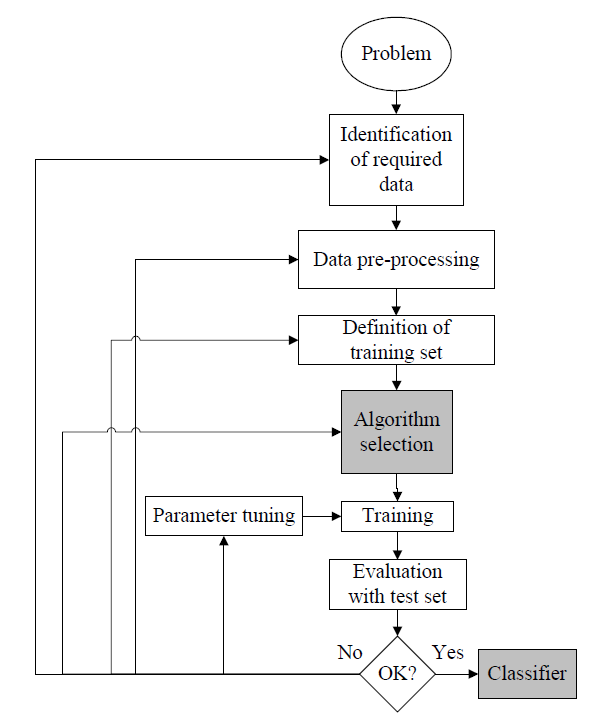
\includegraphics[width=0.8\textwidth]{images/chapter2/supervisedLearning.png}  
    \caption{General process of classification methods. From Kotsiantis et al. \cite{Kotsiantis2007}}
    \label{fig:supervisedLearning}
\end{figure}

\subsection{Decision Trees}

As described by Zaki et al. \cite{Zaki2014}, Decision Tree is a classification model which recursively partitions the data space into two parts. The split can be considered as a hyperplane parallel to one axis of the data space. The process repeats by dividing each new part into two smaller parts, and this process continues until each sub-part mostly contains items of only one of the target classes. The final result of this partitioning process
can be represented by a tree, where each node is a decision concerning which part an item belongs to, and the leaves represent one of the target classes.


As an example of the decision tree partitioning, consider the iris data set with 150 entries of three classes. The items are displayed in Figure \ref{fig:Recurcive2Decision1}, which plots their sepal length and width as X, Y axes. The partitioning process created six different regions, which are divided by lines instead of hyperplains, as in two-dimensional data space the hyperplanes can only have one dimension. Multiple regions might represent one of the targeted classes. The tree representation of the iris data space partition is shown in Figure \ref{fig:Recurcive2Decision2}.

\begin{figure}[!h]
    \hfill{\begin{minipage}{\dimexpr \textwidth-2\fboxsep-2\fboxrule}% maximum allowed
            \centering
            \subfigure[Recursive Splits]{
                \label{fig:Recurcive2Decision1}
                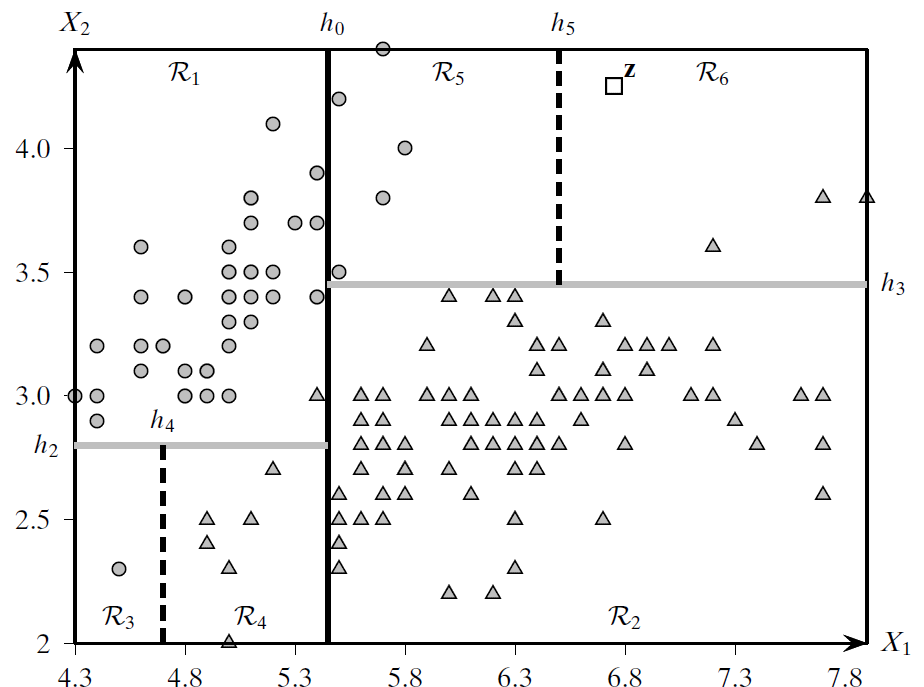
\includegraphics[width=0.8\textwidth]{images/chapter2/RecursiveCut.png}
            }\\
            \subfigure[Decision Trees]{
                \label{fig:Recurcive2Decision2}
                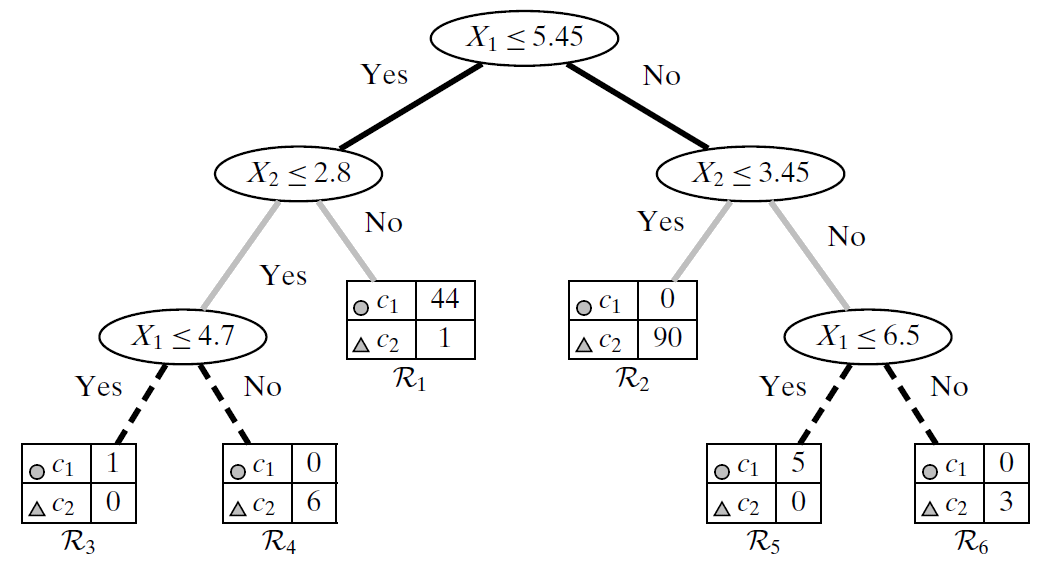
\includegraphics[width=0.8\textwidth]{images/chapter2/DecisionTreeExample.png}  
            }

    \end{minipage}}
    \caption{Decision trees representation for splitting items of the data by creating hyper-plains which are parallel to one of the axes. 
        (a) A two dimensional data set has been split recursively to differentiate between elements of different classes.
        (b) A tree representation for the values of the class limits.
        From Zaki et al. \cite{Zaki2014}}
    \label{fig:Recurcive2Decision}
\end{figure}

C4.5 might be one of the most famous decision tree algorithms for classification \cite{Wu2008}. C4.5 is build on ID3, both of which were introduced by Quinlan \cite{Quinlan2014}. This algorithm relies on information gained to create its tree for classification. In this algorithm attributes with higher normalised information gain are used for decide the splits in the data. The the next highest attribute is used for subpartitioning the data recursively \cite{Quinlan2014}.

This algorithm is superseded by a new version C5.0, which is more efficient as it uses less memory and functions more efficiently and effectively, generating a smaller and more concise decision tree, while it is more general as it can classify more data types than its predecessor. It also incorporates boosting, which means multiple classifier trees can be generated and they will vote for predicting items' classes. Boosting is a bootstrap aggregate (bagging) mechanism which may improve the stability and accuracy of the final result of the classifier \cite{Wu2008}. The last aspect of the algorithm is similar to what is provided by Random Forest algorithm, which creates many decision trees from random subsets of the training data \cite{Breiman2001}.

C4.5 has two drawbacks \cite{Hothorn2006}, the first of which is overfitting, which might be solved by pruning the decision tree to be more general. Two types of pruning can be done on the tree pre-pruning and post-pruning. Pre-pruning is the operation of preventing particular branches from growing when information becomes unreliable. Post-pruning is the operation of cutting branches of a fully grown tree to remove unreliable parts. The second drawback originates from the very nature of the algorithm by selecting attributes with the highest information gain value. This process will become bias to the attributes with a large number of values.

Conditional Inference Tree (Ctree) was introduced by Hothorn et al. \cite{Hothorn2006} to overcome the attribute bias of the information gain based algorithms. This algorithm uses significance to select covariants of attributes. The significance is determined through P-value which is derived from ANOVA F-statistics. During the training phase, all data permutations will be tested to calculate the p-value.

\subsubsection{Rule-Based Classification}

A rule-based classifier uses a set of rules to classify items in a data set. The rules are formalised in the form of IF-THEN clause. The conditions of the IF clause represent the rules that an item should fulfil to be accepted as a particular class. If the rules are ordered and have priority they can be represented in nested IF-THEN-ELSE clauses and might be called decision lists \cite{Witten2011}. 

Figure \ref{fig:ruleBased}a shows a simple data set with items labelled \textbf{a} or \textbf{b}. We can produce multiple variations of rules to classify items in this data set. It is possible to filter out all class \textbf{a} items first then all others remaining will be class \textbf{b}:
If x $>$ 1.4 and y $<$ 2.4 then class = \textbf{a}\\
Otherwise class = \textbf{b}\\

Conversely, if b class items are filtered out the remaining items will be classified as \textbf{a}:
If x $\leqslant$ 1.2 then class = \textbf{b} \\
If x $>$ 1.2 and y $\leqslant$ 2.6 then class = \textbf{b}\\
Otherwise class = \textbf{a}\\


In most cases, rule-based classification systems and decision trees can be used interchangeably; C4.5 provides both decision trees and classification rules \cite{Wu2008}. A decision tree representing the rule-based classifier is shown in Figure \ref{fig:ruleBased}b. The rules above and the decision tree can be considered as an equivalent classifiers, but most of the time people prefer rule-based classifiers on decision trees as they are more intuitive for human understanding \cite{Witten2011}, due to being simpler and more concise \cite{Wu2008}.


\begin{figure}[!h]
    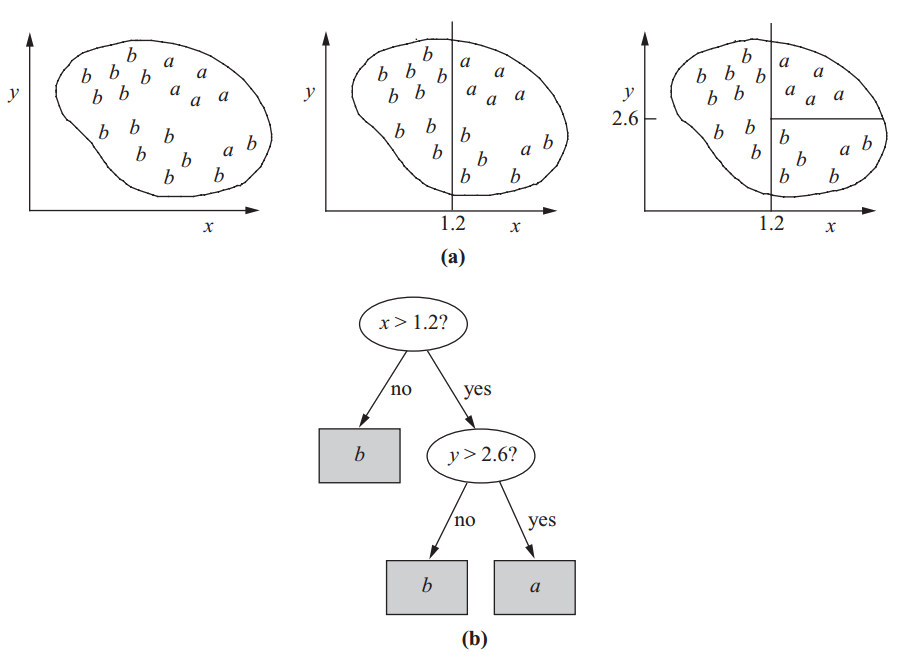
\includegraphics[width=1\textwidth]{images/chapter2/rulebased.png}  
    \caption{Classifying same data set using both rules and a decision tree.
        (a) A two dimensional data sets with items of two classes.
        (b) A tree representation for a rule based classification.
        From Witten et al. \cite{Witten2011}}
    \label{fig:ruleBased}
\end{figure}

Various methods are used to generate rule-based classifiers in different fields of application. The remainder of this section presents more effective samples of these works with a brief explanation of their methodologies.

Rodriguez et al. \cite{Rodriguez2012} used rule-based classification to classify power quality disturbances of signals. They used S-transform to extract features from signals, as this transform can generate variable window size with the ability to preserve phase information during decomposition \cite{Chen1996}. They used leaner and parabolic lines to separate between classes. The separation line is produced using a heuristic function to guarantee maximisation of the number of correctly classified signals from the provided training set.

Chung et al. \cite{Chung2002} use a two-stage classification method to classify power line signals, in the first of which they used a rule-based classifier to differentiate interrupt signals from others, which were then further classified using Hidden Markov Model classifier. The rules of the first stage classifier are created by domain experts relying mainly on the IEEE standards for signal interruption conventions, thus this classifier does not require a training set, as it is a static set of rules that can be calculated directly.

McAulay et al. \cite{McAulay1994} used genetic algorithms to create rule-based systems to identify alphabetical numbers. The system uses a random rule generator to create initial rules, which are enhanced through multiple generations by adjusting the initial rules. However, they notice that genetic algorithms might override even good rules which can identify specific characters. To prevent overriding rules, they introduced the concept of remembering rules for a long time if they succeeded to identify the training set example correctly.

Orriols-Puig et al. \cite{Orriols-Puig2009} used an evolutionary algorithm to create a rule-based classification system in which the system initiates with a set of classifier rules, then evolves online with the environment (new training items) to produce an accurate classification model. They proved that their classification method outperforms other methods (including support vector machine) in classifying data sets with imbalanced class ratios.

Nozaki et al. \cite{Nozaki1996}used fuzzy systems to create a rule-based classifier. Generating fuzzy rule-based classification system requires two phases, first partitioning the patron space into fuzzy subspaces and then defining a fuzzy rule for each of these. Nozaki et al. used a fuzzy grid introduced by Ishibuchi et al. \cite{Ishibuchi1992} with triangle-shaped membership function to generate fuzzy rules from fuzzy subspaces. To enhance the classification results they introduced two procedures, error correction-based learning and significant rule selection. Error correction-based process increases and decreases the procedure of increasing or decreasing rule certainty according to its classification of the items; if a particular rule correctly classified an item its certainty will increase, otherwise, it will decrease accordingly. Significant rule selection is a mechanism to prune unnecessary rules to construct a compact set of a fuzzy rule-based classifier.

As demonstrated above, many domains of computer science and machine learning are used to generate and optimise rule-based classification systems, including expert systems, genetic algorithms, evolutionary algorithms and fuzzy systems. While these classifiers are efficient and effective methods to classify underlying data sets, they require a training data set for rule generation and optimisation. This means a sufficient amount of correctly labelled samples should be available to cover all or most of the aspects and possibilities of situations and characteristics that have to be classified.

The availability of the training data set might not always be an option due to the fact that labelling items is a tedious and laborious undertaking requiring a extensive periods of professionals' valuable time. Experts might know the general rules for classifying items but they cannot identify the attributes of the classes individually due to the complexity of the underlying data sets. Moreover, domain experts might not quite agree on the fine differences between classes, so that it is hard to have a general single view for classifying items in the data set (such as in public goods games case study).

After the training stage these methods create a list of rules that represent the final rule-based classifier model, which might not cover all different opinions for nuanced cases of the classification (i.e. after the training stage, the classifier might lack the required generalisation). As noted previously, the generalisation problem might be solved by using rule pruning \cite{Nozaki1996}. However, this generalisation can be called local, as it depends on the training data, which is probably classified and labelled using expert single views.

Another aspect which is lacking in the presented methods is that they do not consider the classification of temporal data sets, as demonstrated in later sections. However, these methods also require training samples.



\subsection{Support Vector Machine}

\acrfull{svm} is a binary parametric classifier that classifies items by creating a hyperplane between classes. This algorithm tries to find an optimum position for the hyperplane so that it splits the classes with the maximum margin between class items and minimum empirical risk. The items on the edges of the margin are called support vectors, as each item can be seen as a vector. An example of an SVM classifier's hyperplane is shown in Figure 2.4. It can be noticed that in a two-dimensional data set the hyperplane is represented as a line \cite{Muller2001}.

\begin{figure}[!h]
    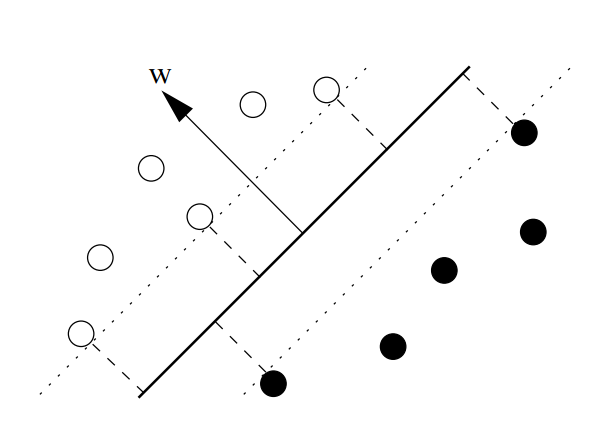
\includegraphics[width=0.6\textwidth]{images/chapter2/SVM.png}  
    \caption{Hyperplane of support vector machine between items of two classes showing vector $w$ and points on the dotted lines are support vectors. From Muller et al. \cite{Muller2001}}
    \label{fig:svmClassifier}
\end{figure}

Assume $D = \{(x_i, y_i)\}^n_{i=1}$ is a data set to be classified. The data set has n items in d dimensions, and each item has a set x of d attributes and y as a class label. For two classes we can assume that y can have one value of 1 or -1. The SVM's hyperplane $h(x)$ equation is defined as $h(x) = w^Tx+ b$. In this equation, w is a d dimensional weight vector and b (bias) is a scalar. The points on the hyperplane equal to 0 ($h(x) = 0$), so that for any $x_i$ if $h(x_i) > 0$ then $y_i = 1$ and if $h(x_i) < 0$ then $_iy = -1$ \cite{Zaki2014}. 

One of the advantages of SVM is that it can use kernel trick. For a data set with nonlinear separation between classes, we can map the d-dimensional items $x_i$ of input space into a high-dimensional feature space using a nonlinear transformation function \cite{Zaki2014}. 


SVM has been used as an elementary stage to create rule-based classifiers. Nunez et al. \cite{Nunez2006} used rule extraction mechanism to extract rules from an SVM model generated via training samples. The rules are constructed using multiple of ellipsoid equations. While these rules might present a good visual illustration for the rules, especially for two-dimensional spaces, these equations have mathematical forms so that the generated rules are not intuitive and easy to understand as stand alone rules. Moreover, the ellipsoids are not one-to-one maps for the actual hyperplanes of SVM, so the rule-based classifiers are not as efficient as their SVM counterparts and they have a higher error rate.



\subsection{K-Nearest Neighbours}
The \acrfull{knn} classifier is a nonparametric lazy classifier. In nonparametric classification the algorithm does not assume any specific distribution for the data sets. Lazy classifiers do not generalise the classification model and calculate the class of the item at the time of testing instead of training, which makes training very efficient by reducing the cost of testing time \cite{Wettschereck1997}. 

KNN estimates items' classes according to their nearest neighbours. The majority of the K nearest neighbours decide the class of the input item. An odd number of for K is selected (between 3 to 9) to prevent ties. The nearest neighbours are decided using one of the distance measures (e.g. Euclidean distance), as shown in Figure \ref{fig:KNN} \cite{Zaki2014}. 

\begin{figure}[!h]

    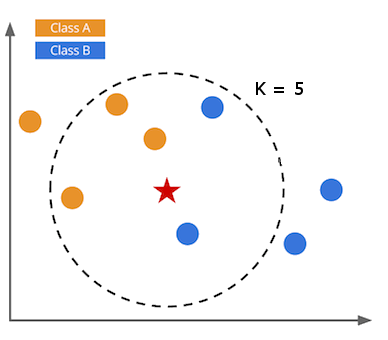
\includegraphics[scale=0.9]{images/chapter2/KNN.png}
    \caption{K-Nearest Neighbour Classification with K = 5}
    \label{fig:KNN}
\end{figure}

To prevent attribute bias due to different magnitudes of values it is strongly preferred to normalise all attributes before classification. Non-numerical attributes can also be used with KNN classification, similar attributes with the K neighbours have zero distance, and different attributes have the distance of 1 \cite{Zaki2014}. 

While this classification algorithm is different from rule-based classifiers, we used a variation of this classification for temporal attributes, as explained in chapter six, as a comparison with our proposed classification algorithm to test the performance difference between the algorithms.


\subsection{Classification Performance Measures}


Multiple methods exist to measure the performance of a classification algorithm and classify a data set into two classes, positive and classified. The terminology was developed in the medical field, where positive denotes the presence of a disease and negative indicates its absence \cite{Fawcett2006}. 

In a test data set D with n instances, a classifier tries to identify the class of instances for binary classifiers, whereby four possibilities exist. These possibilities for any classifier can be demonstrated as a confusion matrix, which is shown in Table \ref{tab:confusionMatrix}, and explained below \cite{Zaki2014}:

\begin{itemize}
    \item \acrfull{tp}: Number of correctly identified positive cases by the classifier.
    \item \acrfull{fp}: Number of incorrectly identified cases as positive but their true labels are negative.
    \item \acrfull{tn}: Number of correctly identified negative cases by the classifier.
    \item \acrfull{fn}: Number of incorrectly identified cases as negative but their true labels are positive.
\end{itemize}

\begin{table}[!h]
    \centering
    \begin{tabular}{l|l|c|c|c}
        \multicolumn{2}{c}{}&\multicolumn{2}{c}{True diagnosis}&\\
        \cline{3-4}
        \multicolumn{2}{c|}{}&Positive&Negative&\multicolumn{1}{c}{Total}\\
        \cline{2-4}
        \multirow{2}{*}{Screening test}& Positive & TP & FP & $a+b$\\
        \cline{2-4}
        & Negative & FN & TN & $c+d$\\
        \cline{2-4}
        \multicolumn{1}{c}{} & \multicolumn{1}{c}{Total} & \multicolumn{1}{c}{$a+c$} & \multicolumn{1}{c}{$b+d$} & \multicolumn{1}{c}{$N$}\\
    \end{tabular}
    \caption{Confusion Matrix}
    \label{tab:confusionMatrix}
\end{table}

To measure the overall performance of a classifier directly from the confusion matrix we can calculate the accuracy and error rates. The accuracy of a classifier is the fraction of correctly classified instances so that: $Accuracy = \frac{TP + TN}{n}$. In contrast, the fraction of all misclassified instances comprise the 
error rate which is: $Error Rate = \frac{FP + FN}{n}$ \cite{Fawcett2006}.

To measure class-specific performance we can use recall and precision. Recall is the ratio of correctly predicted number of a class labels to the real number of instances of that class in the data set. Recall for the positive instances in the data set is called sensitivity. The sensitivity is the ratio of true positive to the real number of positive cases in the data set so that $sensitivity = \frac{TP}{TP + FN}$. Precision is a class-specific accuracy; it is the ratio of the number of correctly predicted instances of a class to the number of predicted instances of the same class. A specific case of precision for the negative class is called specificity. The specificity is the ratio of true negative to the real negative cases in the data set so that $specificity = \frac{TN}{TN + FP}$ \cite{Fawcett2006}.

For a classifier, there is a trade-off between recall and precision; maximising one of them might cause the other to decline. Consequently, measures are introduced to overcome this problem and create a balance between these two measures. F-measure is computing the harmonic mean of the classes' recall and precision \cite{Zaki2014} so that:
\begin{equation*}
    F=\frac{2}{\frac{1}{precision} + \frac{1}{recall} } = \frac{2 \times precision \times recall}{precision + recall}
\end{equation*}


\acrfull{auc} of \acrfull{roc} is a measure used to calculate the performance of machine learning algorithms such as classification \cite{Bradley1997} . The ROC curve is a graph of the true positive and false positive rates of the predicted classifier's result compared to the real class for each item. Figure 2.6 shows ROC curves for different algorithms with various performances. AUC is the area under the ROC curve plotted as a performance result of the classifier. Methods of calculating AUC vary according to the nature of application and available data. The multi-class AUCs are calculated using the equations of \cite{Hand2001}. $auc = \frac{2}{c(c-1)}\sum aucs$. Where c is number of classes and aucs is a set of auc between any two classes.

\begin{figure}[!h]
    
    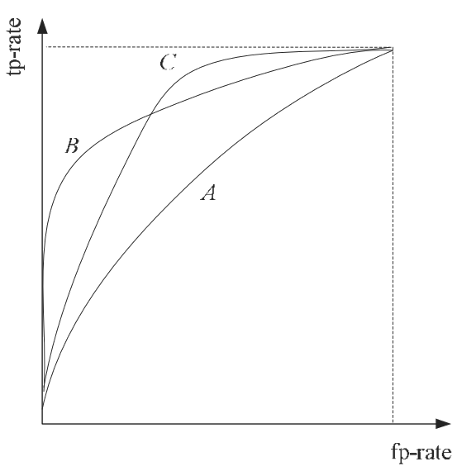
\includegraphics[scale=0.4]{images/chapter2/AUC.png}
    \caption{Receiver operating characteristic (ROC) curves for various classifiers. From \cite{Dietterich2010}}
    \label{fig:ROC}
\end{figure}

\section{Clustering}

Unsupervised machine learning methods aim to find patterns or groups (clusters) in data sets so that the most similar items in the data set will be gathered in the same cluster, and dissimilar items will be in different clusters. The task of clustering is required in many fields, especially when little information is known about the data sets, and field experts have few assumptions about it. Examples of fields in which clustering is required include data mining, pattern recognition, decision making, document retrieval and image segmentation \cite{Jain1999}.

In this thesis, multiple clustering algorithms are used to cluster items of each time point in temporal data. Each time point was used separately, so there is no time effect on the clustering because each time point is treated as a separate data set. This clustering process is part of the proposed method to measure changes over time in temporal data (as presented in chapter four). We also used clustering multiple temporal clustering algorithms as a comparison with our proposed classification method (chapter six).

Figure \ref{fig:Clustering} shows the main steps of a clustering method. It can be noticed that unlike supervised methods, clustering methods do not have training data set to generate their model. Instead, they entirely depend on the given features of the items in the data set to group them into clusters. 

\begin{figure}[!h]
    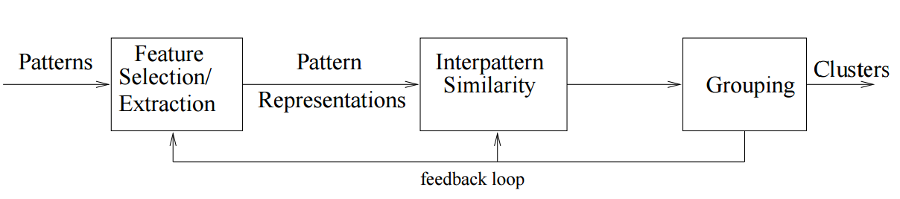
\includegraphics[scale=0.4]{images/chapter2/ClusteringSteps.png}
    \caption{General steps of clustering methods. From \cite{Jain1999}}
    \label{fig:Clustering}
\end{figure}

The first step in any clustering task is feature selection/extraction. Feature selection refers to selecting a group of features (attributes) of the original data set which are most effective and representative for the instances or items which have to be clustered. Feature extraction is the process of deducing new features by transforming existing ones to obtain more effective features. The aim of feature selection and extraction is to obtain an effective and efficient clustering method by creating better quality of clusters in shorter computation time \cite{Jain1999}.

The second step is detecting pattern similarity by finding the distances between items in the data set. Multiple distance measures are available to measure the similarity between any two points in a hyperspace of features like Euclidean and Manhattan distances and correlation coefficients \cite{Jain1999}.

The next step is the actual clustering process to identify patterns in data sets using one of the available clustering algorithms. There are multiple clustering algorithms which can be classified into four types Centroid-based clustering, Density-based clustering, Fuzzy clustering and Hierarchical clustering \cite{Zaki2014}.

The last step is feedback or clustering evaluation. There are many ways to evaluate the results of clustering algorithm, including using external clustering validity indices to compare generated clusters with the true classes of the items or using internal clustering validity to evaluate the structure of the clusters and the similarities between items of one cluster compared with dissimilarities with items of different ones \cite{Jain1999, Zaki2014}.


\subsection{Centroid-Based Clustering}

Centroid-based or representative-based clustering is a method of finding the best k clusters of items in the D data set. Each cluster contains a representative point which might be called centroid \cite{Zaki2014}. Two examples of centroid-based clustering discussed below are K--means and PAM clustering methods.

\subsubsection{K--means Clustering}

K--means clustering is partitional-based and produces k clusters, minimising the distance between the centre of the cluster and cluster members. The criterion used to calculate the quality of the cluster is the sum of squared errors to the centroid. The aim of the algorithm is to find centroids that minimise the sum of squared error for all clusters \cite{Zaki2014}. 

The process starts by assigning k random items as centroids, after which each item is appointed to a cluster with the nearest centroid to it. The location of the centroid is updated according to the existing items in the cluster. The process of assigning instances to clusters and updating centroids is reiterated until convergence (i.e. the centroids stabilise) or a fixed number of iterations has been reached \cite{Jain1999}.  

K--means works as a greedy optimisation algorithm so that it might converge to local optima \cite{Zaki2014}. Moreover, using the sum of squared error as a criterion for finding better clusters makes K--means sensitive to outliers, so that extreme values might distort the distribution of the data \cite{Jain1999}. 

\subsubsection{PAM Clustering}

\acrfull{pam} clustering is another centroid-based technique, but unlike K--means it uses actual instances of the data set as representatives for the clusters instead of virtual centroids. It uses a similarity measure to identify members of a cluster. The members most similar to a medoid are considered in the same cluster so that the sum of squared errors can be used with PAM algorithm to identify the quality of clusters \cite{Kaufman1990}.

Similar to K--means, PAM algorithm starts with random k set of medoids, then each instance is registered as a member of a cluster according to its similarity distance from the medoid. The sum of squared errors is calculated for the current set of medoids. In the original algorithm, different instances are selected as nominees for medoids to optimise the initial state, and the sum of squared errors is calculated according to the selected instances \cite{Kaufman1990}. If the selected instances perform better than the original set of medoids, then they will be replaced with the new ones. This process can be repeated multiple times until convergence. However, due to the large time requirement and complexity of this method, it is usually used only for small data sets, and for larger data sets a modified version of the original version is preferable to find optimum medoids in an acceptable time frame \cite{Ng2002}. 

\subsection{Fuzzy Clustering}

Fuzzy sets are used in fuzzy logic and can be considered as a generalisation of set theory. An element can be a member of a particular set or not in set theory, while in fuzzy set theory an element can have a gradual transition membership between sets. Hence, fuzzy clustering uses the fuzzy set to allow an instance to be in more than one cluster at the same time \cite{Wang2006}. 

The most well known and used fuzzy clustering is fuzzy c--means algorithm, developed by Dunn \cite{Dunn1973a} and later improved by Bezdek \cite{Jain1999} who introduced the concept of the fuzzifier parameter \textbf{m}. This parameter, also called 'fuzziness index', is used to control the fuzziness of the membership of each item in the data set. Usually, m = 2 is used without any particular theoretical basis for this choice. For m = 1 the fuzzy c--means will behave as k--means algorithm, and the fuzziness of the system increases with the larger value of m parameter \cite{Bezdek1981}. 

The fuzzy c--means algorithm has a similar approach as k--means algorithm. It requires a predefined number of clusters. Both algorithms start with random initialization of the cluster centres so c--means might have the same problem as k--means by converging to local optima. The result of the cmean algorithm is expressed as a membership percentage of each instance to the available clusters. This fuzzy membership clustering can be converted into hard clusters by choosing a cluster for each item with the highest membership ration \cite{Wang2006}.

\subsection{Hierarchical Clustering}

Hierarchical clustering is a method to group instances of a data set into a series of nested clusters or a tree of clusters called a dendrogram, which represents the similarity level between instances in the data set. An example hierarchical clustering is shown in Figure \ref{fig:Hira}. The figure shows a simple two-dimensional data set with three distinctive clusters. The data set is represented as in a hierarchical clustering model using a dendrogram. The dendrogram can be cut at any level (represented as a dotted horizontal line) to separate different patterns of the data set \cite{Jain1999}. The level of the cutoff line is subjective and may vary from one data set to another. Cutting a dendrogram from a higher level produces fewer patterns (clusters) \cite{Wang2006}.

\begin{figure}[!h]
    \hfill{\begin{minipage}{\dimexpr \textwidth-2\fboxsep-2\fboxrule}
            \centering
            \subfigure[Data set]{
                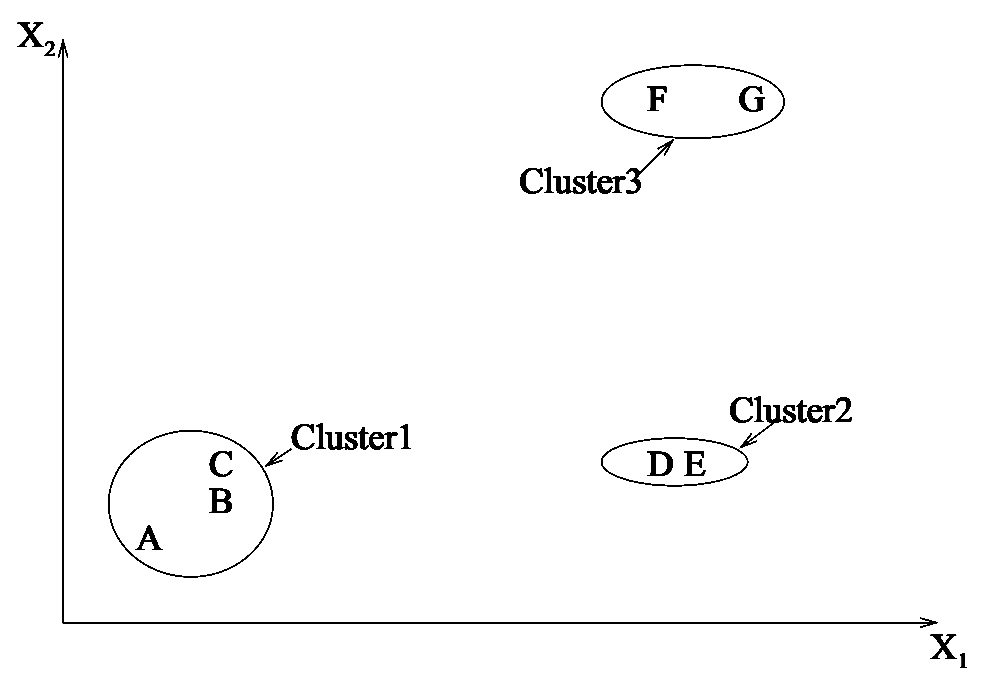
\includegraphics[width=0.7\textwidth]{images/chapter2/hira1.png}
            }\\
            \subfigure[Dendrogram of the data set]{
                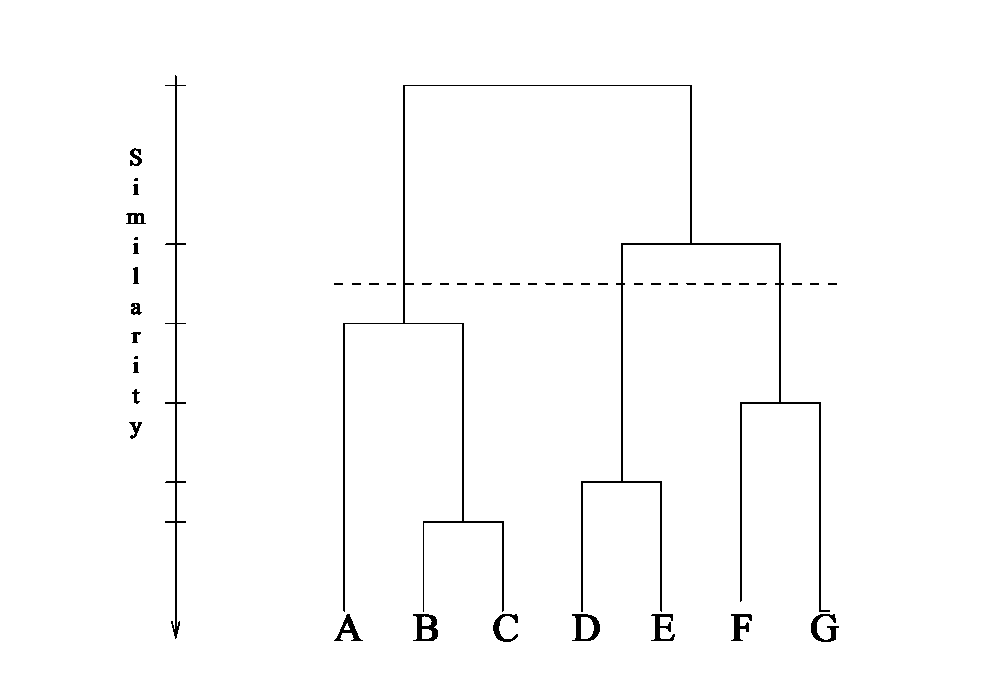
\includegraphics[width=0.7\textwidth]{images/chapter2/hira2.png} 
            }
            
    \end{minipage}}
    \caption{A simple data set with a possible dendrogram for hierarchical clustering algorithm. 
        (a) Two dimensional data set with three obvious different groups.
        (b) A dendrogram representation for a hierarchical clustering of the previous data set
        From \cite{Jain1999}}
    \label{fig:Hira}
\end{figure}

Based on the internal functioning of the hierarchical clustering algorithm, they can be divided into divisive and agglomerative types. The divisive method starts by assigning all instances into one cluster then partitions that cluster into two smaller clusters according to the similarities between instances. The process of sub-dividing each subcluster into another two clusters continues until each cluster contains single instance. In contrast, agglomerative hierarchical clustering starts by assigning each instance of the data set as a cluster, then starts to combine two most similar clusters into a single bigger cluster. This process is repeated recursively until a single cluster is achieved or a certain number of clusters are reached \cite{Zaki2014}.

Whether divisive or agglomerative approach is used, a prerequisite to begin clustering is a proximity matrix, a symmetric matrix containing the similarity between every point in the data set using a distance function. This matrix is updated after each iteration to reflect the status of the data set under the method of clustering. The distance function can be Euclidean, Manhattan or any other distance function \cite{Zaki2014}. Sections shows how time-based distance measures can be used to cluster temporal data sets.

To determine the similarity between clusters using proximity matrix in agglomerative method, one of the available linkage methods can be used \cite{Wang2006}:

\begin{itemize}
    \item Single linkage: calculates the minimum distance between any items of two different clusters.
    \item Complete linkage: calculates the maximum distance between any items of two different clusters.
    \item Average linkage: calculates the average distance between all items of two different clusters.
    \item Centroid linkage: calculates the distance between centre of two different clusters.
\end{itemize}

Due to the time complexity hierarchical clustering can not be used with very large data sets which can not fit the memory. Moreover, the nature of the algorithm do not allow to reconsider the previous steps of the recursive clustering operation (dividing or joining) in contrast with the other clustering technique which we see before \cite{Wang2006}. 


\subsection{Clustering Validation}

Many clustering methods exist to be used in different situations according to the underlying data to be analysed and clustered. There are many methods to assess clustering results and their initial configurations, which can be categorised into three main types: clustering tendency, cluster stability and cluster evaluation \cite{Zaki2014}. 

Clustering tendency or clusterability assesses the suitability of the data for clustering. The aim is to determine that the data has meaningful patterns to be clustered. The spatial histogram method for cluster tendency creates a histogram for the input data set and distance distribution by calculating the pairwise distance between data points. An example of non-clusterable data is uniform instances of a data set, as shown in Figure \ref{fig:uniformData} \cite{Zaki2014}. 

\begin{figure}[!h]
    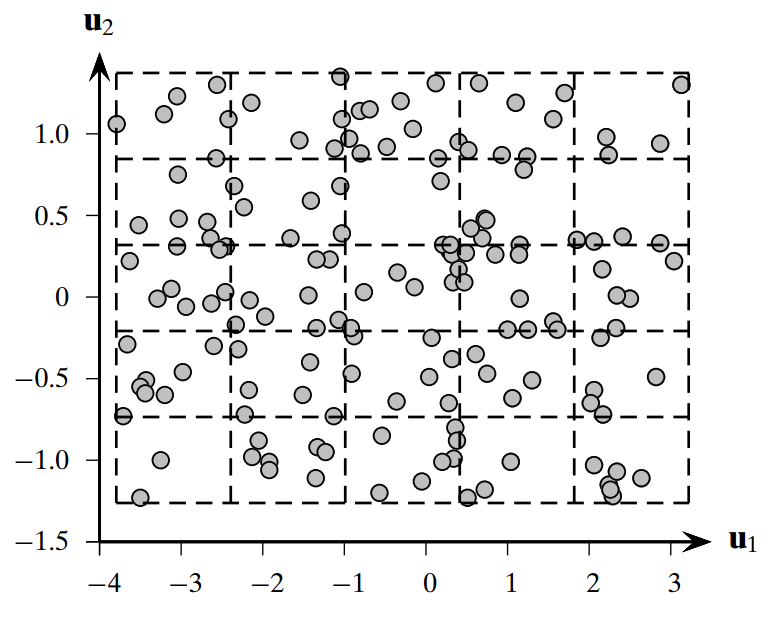
\includegraphics[scale=0.33]{images/chapter2/uniformData.png}
    \caption{An example of uniform data which can not be clustered. From Zaki et al.\cite{Zaki2014}}
    \label{fig:uniformData}
\end{figure}

Cluster stability is concerned with the initial parameters of clustering algorithms, like the number of clusters in K--means. The aim of this method is to determine the optimum initial parameters for the clusters, so that the cluster of different samples of data from the same underlying population guarantee comparable results. Methods of determining the stability of clusters include generating perturbed versions of the data set, using distance functions (e.g. Euclidean) and similarity measures like Rand index \cite{VonLuxburg2010}.

Clustering evaluation can use cluster validity indexes to evaluate the quality of the produced clusters. This task can be further divided into three categories \cite{Halkidi2002a, Halkidi2002, Zaki2014}:

\begin{itemize}
    
    \item \textbf{External}: External validation derives the estimation for the quality of the generated clusters from sources outside the data set. The most general case is using true labels of items, provided by field experts.
    
    \item \textbf{Internal}: Internal validation derives the estimation for the quality of the generated clusters using the structure of the data and the clusters. It computes the compactness of the clusters and the separation of clusters from each other.
    
    \item \textbf{Relative}: External validation compares between the results of two different clusterings for the same data set. The clusterings might be generated using different clustering algorithms, or the same clustering algorithm with different initial parameters.
    
\end{itemize}

The following subsections focus on the cluster validity indices, especially those used in this thesis.

\subsubsection{External Criteria}
External criteria validate the results of clustering based on some predefined structures of the data which is provided from an external source. The most well-known example of structural information is labels for the data provided by experts (called true classes). The main task of this approach is to determine a statistical measure for the similarity or dissimilarity between obtained clusters and labels \cite{Halkidi2002a, Rendon2011}. According to the methods incorporated in the external criteria, they can be divided into three types: pairwise measures, entropy-based measures and matching based measures \cite{Zaki2014}. 

As mentioned previously, the four types of classification guesses evaluation are true positive, true negative, false positive and false negative. These terms are used in the terminology of external cluster validity, especially when using pairwise measures, but with slightly different meanings to enable the evaluation of clusters in the same manner as classification \cite{Zaki2014}:
\begin{itemize}
    \item True Positives \textbf{TP}: Any two instances with the same label that are in the same cluster.
    
    \item False Negatives \textbf{FN}: Any two instances with the same label that are not in the same cluster.
    
    \item False Positives \textbf{FP}: Any two instances with different labels that are not in the same cluster.
    
    \item True Negatives \textbf{TN}: Any two instances with different labels that are not in the same cluster.
    
\end{itemize}

In this thesis, we use various external cluster validity indices to determine differences between a reference of behaviour for items in a temporal data and clusters of items in each time point. The method is discussed in more detail in chapter three and implemented in chapter four for public goods games and chapter six for stock market data. The used criteria in the thesis are listed below:

\textbf{Jaccard Coefficient: }
This coefficient is a pairwise measure representing the degree of similarity between clusters. With this coefficient, each cluster is treated as a mathematical set, and the coefficient value is calculated by dividing the cardinality of the intersection of the resultant cluster with the prior cluster to the cardinality of the union between them \cite{Vendramin2010}:
\begin{equation*}
Jaccard = \frac{TP}{TP + FP + FN}
\end{equation*}

With a perfect clustering, when false positives and false negative equal to zero, the Jaccard coefficient value equals 1. This measure ignores the true negatives and only focuses on the true positives to evaluate the quality of the clusters \cite{Zaki2014}. 

\textbf{Rand Statistic: }
The Rand statistic measures the fraction of true positives and true negatives over all point pairs; it is defined as
\begin{equation*}
Rand = \frac{TP + TN}{N}
\end{equation*}
Where N is the total number of instances in the data set. This measure is similar to Jaccard Coefficient, so its value equals 1 in perfect clustering \cite{Zaki2014}.


\textbf{\acrfull{fm}:}
FM define precision and recall values for produced clusters \cite{Fowlkes1983}
\begin{equation*}
FM = \sqrt{prec. recall} = \frac{TP}{\sqrt{(TP + FN)(TP + FP)}}
\end{equation*}
Where $prec = \frac{TP}{TP + FP}$ and $recall = \frac{TP}{TP + FN}$. For the perfect clustering this measure equals 1 too \cite{Zaki2014}.



\textbf{\acrfull{vi}: }
This index measure is based on contingency table which is a matrix with $r \times k$ , where $r$ is number of produced clusters and $k$ is the number of externally provided clusters. Each element of this matrix contains a number of agreed instances between any two clusters of the externally provided and produced clusters. As introduced by Meila \cite{Meila2007a}, this index calculates mutual information and entropy between previously provided and produced clusters derived from the contingency table:
\begin{equation*}
VI(C,T) = 2H(T,C)- H(T)- H(C)
\end{equation*}
Where $C$ is produced clusters, $T$ is ground truth clusters, $H(C)$ is entropy of $C$ and $H(T)$ is entropy of $T$ \cite{Zaki2014}.




\subsubsection{Internal Criteria}
Internal criteria measure the 'goodness' of clusters for the data by extracting information from data and clusters alone, such as the compactness of data points inside one cluster and the separation of clusters from each other \cite{Rendon2011}. These criteria were used as part of the cost function, to determine the quality of the selected classification rules in each time point, and to compare different clustering algorithms' performances, as presented in chapter six.


\textbf{Dunn Index: }
This index calculates the ratio of minimum distance between clusters to the maximum distance between any two instances of the same cluster \cite{Dunn1973}:
\begin{equation*}
Dunn = min_{1\leqslant i \leqslant c} \left \{ min \left \{ \frac{d(c_i, c_j)}{max_{1\leqslant i \leqslant k(d(X_k))}} \right \} \right \}
\end{equation*}
Where $c_i, c_j \in c$ of size $m$ and the maximum distance can be computed from the mean or between all pairs. A larger value for Dunn index means, better clustering output, because it means that the closest instances between two clusters are larger than the distance between two farthest instances in the same cluster \cite{Zaki2014}.


\textbf{\acrfull{db}:}
This measure is introduced by Davies et al. \cite{Davies1979a}. It calculates intera cluster compactness and inter cluster separation by producing the ratio of spreading sample points around mean (i.e. variation) to the distance between mean of clusters \cite{Rendon2011}. 
\begin{equation*}
DB = \frac{1}{k} \sum_{i=1}^{k}\sum_{j=1}^{k}\max_{i\neq j }\left \{ \frac{s_{\mu_i} + s_{\mu_j}}{\delta(\mu_i, \mu_j)} \right \}
\end{equation*}
Where $k$ is number of clusters, $ s_{\mu_i}$ and $s_{\mu_j} $ are the spread of points around any two clusters cluster mean ''Centroid'', and $\delta(\mu_i, \mu_j)$ denotes the mean of both clusters.

A smaller value of this measure indicates better the clustering, as in such cases the clusters are well separated and each cluster is well represented by its mean; in other words, larger values mean better compacted instances in the clusters and clusters that are well separated from each other \cite{Zaki2014}.


\textbf{\acrshort{sd}: } This measure is introduced by Halkidi et al. \cite{Halkidi2000}. It calculates the average scattering for clustering and total separation among clusters. 
\begin{equation*}
SD = a \times Scatter + Distribution 
\end{equation*}
Where $a$ is a weighting factor equal to the maximum distance of two instances in the data set. The $Scatter$ indicates the average compactness of clusters. A smaller value of $Scatter$ is a signal for a compact cluster, and its the value increases for less compact clusters. The $Distribution$ is the measure of the total separation between clusters. A larger value $Scatter$ indicates better clustering and a smaller value of this term indicates greater proximity between clusters to each other. $Scatter$, and $Distribution$ have different ranges so that $a$ (the weighting factor) is important to maintain the balance between them. As SD measure is a total of $Scatterer$ and $Distribution$ so that the smaller SD value indicates better clustering \cite{Halkidi2000}.


\textbf{\acrshort{sdwb}:} This measure is introduced by Halkidi et al. \cite{Halkidi}. The S\_Dbw index is similar to SD index as it measures the intracluster and intercluster variances \cite{Rendon2011}. The definition of S\_Dbw indicates that both criteria of ''good'' clustering (i.e. compactness and separation) are properly combined, enabling reliable evaluation of clustering results. 
\begin{equation*}
S_Dbw = Scatter + Dens_bw
\end{equation*}
 As with SD, the $Scatter$ indicates the average compactness of clusters, smaller $Scatter$ value indicating a compact cluster, with an increased value for less compact clusters. Dens\_bw(c) indicates the inter-cluster density by calculating the average number of points between the clusters in relation with density within clusters. Thus a small value of Dens\_bw means good separation among clusters. As in SD, a smaller value of this measure is an indication of well defined clustering \cite{Halkidi}.


\subsubsection{Relative Criteria}

Relative criteria are used to compare between two clusterings with same data and clustering algorithm but different initial parameters, like number of clusters \cite{Halkidi2002}. These criteria mostly use internal clustering validity indices like Dunn index and Davies–-Bouldin Index to compare between clusterings' initial parameters \cite{Jain1988}. On the other hand Vendramin et al. \cite{Vendramin2010} proposed a novel method to compare relative criteria, using external cluster validity indices like Jaccard and Rand.



\section{Temporal Data Analysis}

Temporal data analysis is concerned with mining and analysing sequential data sets \cite{Laxman2006}. A sequential data set is ordered according to some index. A special case of sequential data is temporal data, which is ordered according to a time reference. According to Han et al. \cite{Han2006}, ''A time-series database consists of sequences of values or events obtained over repeated measurements of time.''. In this thesis, we use the terms ''time series'' and ''temporal data'' interchangeably. Sequential data sets can be used in applications to study protein order series, DNA sequence and lists of moves in a chess game. Examples of temporal data include stock market data and public goods game data set. Data streams can be considered as a special case of temporal data with an endless sequence of flowing data, such as satellite remote sensor, data from electric power grids and telecommunications data \cite{Han2006}.

In the following subsections we discuss methods to measure changes in temporal data as well as classifying and clustering them.

\subsection{Measuring Changes in Temporal Data}

Spiliopoulou et al. \cite{Spiliopoulou2006} introduced the \acrshort{monic} model, which finds cluster transition over accumulating data sets, providing an ageing function for clustering data that prioritises new records over old ones and eliminates records older than two time points. Matching for clusters in one time point to the next one is carried out by passing a threshold that determines normalised maximum number of records that exist in both matched clusters in the two time points. This model defines two kinds of transitions, external and internal. In external transition, clusters may survive, split, be absorbed, disappear or emerge, while in internal transition clusters can change in size, compactness or location.

According to MONIC, each cluster has a lifetime, which is the number of time points throughout which it can survive. Longer cluster lifetimes enable more predictable clustering while short lifetimes lead to volatile and unpredictable clustering.


It can be observed that this model relies on \gls{accumulateddata} over time to detect cluster matches, therefore it cannot be used with non-accumulated data. Moreover, it emphases the measurement of cluster changes and cannot detect changes in cluster membership for individual items clustered over time points.



Gunnemann et al. \cite{Gunnemann2011a} introduced a method which traces cluster evolution as change in behaviour types indicated by the value of objects (e.g. persons) in high-dimensional data sets. Different types of mapping function were introduced to map clusters according to their values in different dimensions and subspaces instead of object identifier.

Using this method cluster evolutions were detected and counted in the forms of emerge, disappear, converge and diverge. Moreover, the loss and gain of dimensions of subspace clusters were calculated.

This method counts the number of various changes that occur to clusters of any high dimensional data set, but it lacks to any mean by which to quantify the changes themselves; in other words, there is no indication of the quantity of change that happens to any cluster in two consecutive time points.



Hawwash et al. \cite{Hawwash2012a} proposed a framework for mining, tracking and validating clusters in a data stream using statistical cluster measures like cardinality, scale and density of clusters to detect milestones of clusters change and monitor the behaviour of cluster.

This framework targets accumulative clustering on data streams, but instead of using fixed-time window for clustering it uses milestones to detect the next-best clustering time.

Hawwash et al. \cite{Hawwash2012a} used a linear model in their metrics, which cannot represent real-life situations. They made this concession due to time limitations and the memory complexity of higher degree models. With some enhanced models this method could be profitably used to determine critical time points in the data stream clustering and to track clusters behaviour in general using statistical measures for representative numbers pertaining to the situation of clusterings.



Kalnis et al. \cite{Kalnis2005} introduced a method to discover moving objects in the snapshots of spatio-temporal data using cluster mapping function, treating clusters as sets and calculating the cardinality ratio of intersection for each two time constitutive clusters over their union; if the ratio passes a certain threshold the cluster is considered to be a moving cluster.

This method detects move in overall clusters and provides visual aids enabling human experts to grasp changes in the underlying data \cite{Ntoutsi2011, Bottcher2008}. This method is excellent for tracking moving cluster change \cite{Ntoutsi2009} , but it still lacks a method to quantify the magnitude of change for overall clustering objects.




Aggarwal \cite{Aggarwal2005} introduced a new method to detect changes for single clusters in the data streams that also works for snapshots of data as special cases. This method uses forward and reverse time slice density estimates based on fixed length time window to calculate velocity density at time and space dimensions.

By calculating velocity density three types of change can appear on the clusters in evolving data streams: 1) they may coagulate if the value passed a user specified threshold; 2) they may decay if the value does not pass the threshold; or 3) they may shift their location to another. This method is particularly germane to visually understanding the characteristics of underlying data.


In summary, the previously mentioned methods: 1) are mostly designed to work with data streams or snapshots of spatio-temporal data sets; 2) detect changes inside data by monitoring cluster change in terms of split, absorbed, disappear and emerged etc., which is a good indication for detecting existence of change, but which does not specify the magnitude of change. Our aim is to create a simple factor (scalar) to express the magnitude of change among members of clusterings in temporal data sets.


\subsection{Temporal Classification}

Temporal and sequence classification is an automatic system that assigns one of the predefined classes to the time series or sequence input \cite{Laxman2006}. Many temporal classifications have been introduced that reuse traditional classification algorithms in terms of criteria and measurements crafted for temporal data. Three main methods exist for classifying temporal data set: distance--based, feature extraction--based and model--based \cite{Amr2009,Laxman2006}.

Wang et al. \cite{Wang2005} proposed a rule-based classification method for categorical and high-dimensional data sets that rely on calculating frequent item sets using frequent pattern mining and association rules, then using the highest confidence sets covering rules for grouping according to rule heads (class labels). This method has been found to result in an efficient and accurate rule-based classifier, but it might produce a very large number of rules, as they are extracted from association mining, which might be hard for humans to follow and comprehend. Moreover, to create the frequent item test, it is required to have training data sets, which might be expensive and labour intensive to acquire and deploy.

It is possible to use traditional classification algorithms (non-temporal) to classify temporal data set by using distance measures specially designed to evaluate distances in a temporal data set. Many temporal supervised and unsupervised algorithms use \acrfull{dtw} \cite{Berndt1994} to align between two sequences or time series and find the distance between them. This method was originally used in speech recognition to identify human speech patterns \cite{rabiner1993fundamentals}. 
 

\begin{figure}[!h]
    \centering
    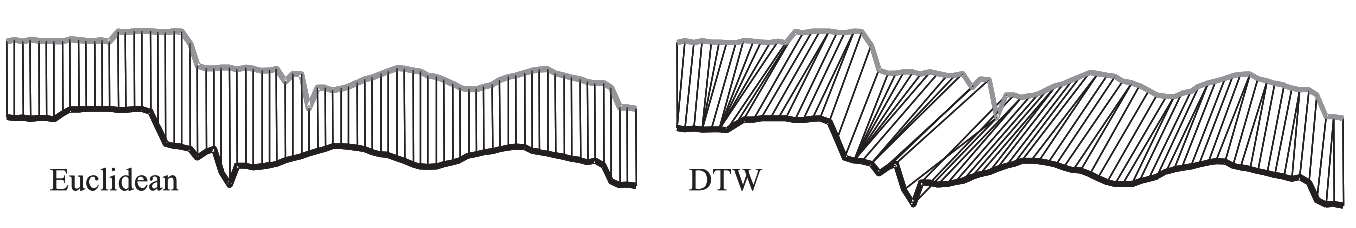
\includegraphics[width=1\textwidth]{images/chapter2/DWtvsEuclidean.png}
    \caption{Difference between time alignment and Euclidean distance of two time series. Aligned points are indicated by arrows. From Keogh et al. \cite{Keogh2005}}
    \label{fig:DWtvsEuclidean}
\end{figure}


Dynamic time wrapping tries to find the best match between two time series to calculate the smallest distance between them, unlike Euclidean distance, which uses the one-to-one mapping between the same time points regardless of any time shift. Figure \ref{fig:DWtvsEuclidean} compares these two distance measures. Dynamic time wrapping creates wrapping matrix which consists of Euclidean distances between every two points in both time series; then a local cost function finds the shortest path between two time series that represents the best match. Dynamic time wrapping has been implemented successfully in numerous temporal classification and clustering methods, but it has a drawback in using heuristic methods, which are inefficient due to searching for the best path in the wrapping matrix \cite{Keogh2005}. The wrapping matrix and time wrapping distance between two time serris are shown in Figure \ref{fig:timewrapIllustration}.

\begin{figure}[!h]
    \centering
    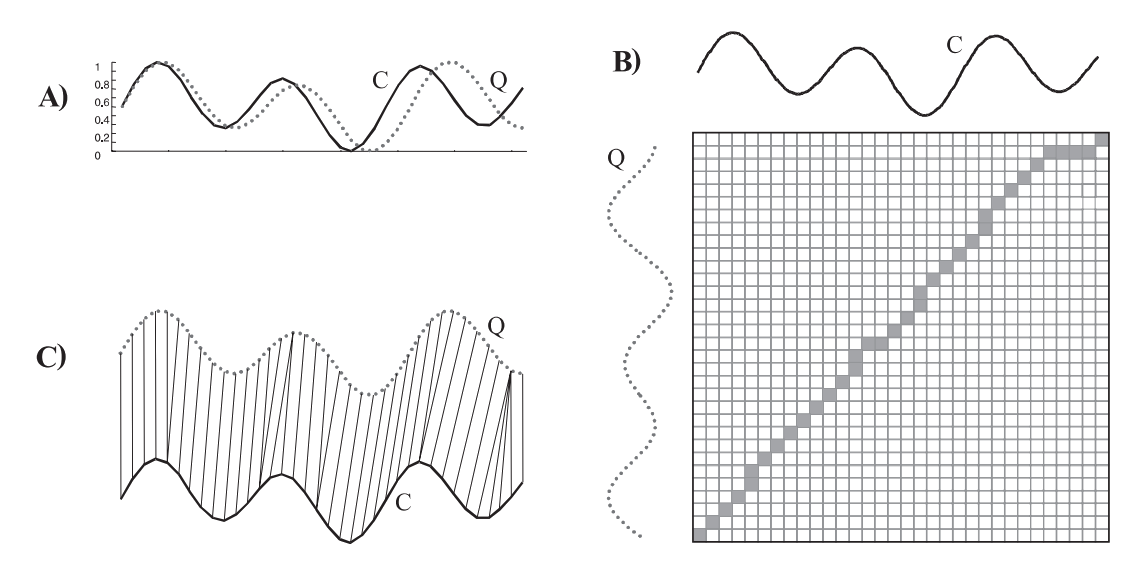
\includegraphics[width=1\textwidth]{images/chapter2/DTWIlustration.png}
    \caption{Calculating the distance between two time series using wrapping matrix. 
        (a) Two similar but out of phase sequences. 
        (b) Finding the optimal path (minimum distance) between the sequences which causes time wrap alignment between different time points of them.
        (c) The resulting alignment.
        From Keogh et al. \cite{Keogh2005}}
    \label{fig:timewrapIllustration}
\end{figure}



\begin{figure}[!h]
    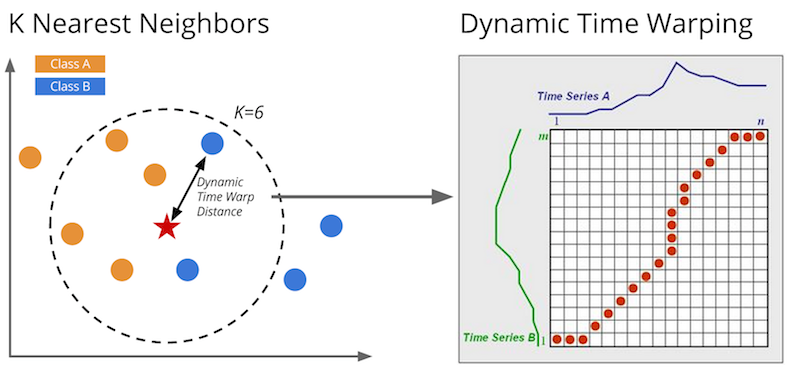
\includegraphics[scale=0.8]{images/chapter2/KNN_Temporal.png}
    \caption{K-Nearest Neighbour using dynamic time wrapping for time series classification. From Regan \cite{Regan2014}}
    \label{fig:KNN_Temporal}
\end{figure}

Distance-based K-Nearest Neighbours classification method (KNN) is used with temporal and sequential data with Euclidean distance measure \cite{Wei2006}. However, for complex time series, Euclidean distance is sensitive to the time fluctuation; thus DTW has been used \cite{KajanLaszl2006}. Figure \ref{fig:KNN_Temporal} illustrates temporal KNN operation.




It is possible to use feature extraction in order to extract useful features from time series so that it becomes possible to use traditional classification methods to classify temporal data. Agrawal et al. \cite{Agrawal1993a} proposed the use of the \acrfull{dft} to transform a sequence from the time domain to the frequency domain. Using DFT allows selection of the most important frequencies then representing them back in the original dimensional space. The DFT has an important property as it can ignore shifts and find similar sequences because the Fourier coefficient is invariant for shifts.


Chan et al. \cite{Chan1999} used \acrfull{dwt} to translate each time series from the time domain into the time/frequency domain. This transformation is linear as it changes the original time series into various frequency components in a lossless transformation. The sequence is then represented by its features, expressed as wavelet coefficients. Only a selected number of coefficients are necessary to represent the original time series, which allows a better and efficient use of the available classification algorithms.


Douzal-Chouakria et al. \cite{Douzal-Chouakria2012} used classification trees to classify time series data by introducing new splits for the tree nodes using time series proximities, relying on adaptive metrics considering behaviours and values. Other methods use SVM as a temporal data classifier using different kernels \cite{Sitaram2007}.

Model-based classifiers can also be used for temporal and sequential classifications, like Naive Bayes sequence classifier \cite{Tseng2009} and Hidden Markov Model \cite{Oates1999}. In the training step, the parameters of the model are created and trained depending on some assumptions, and a set of parameters describing probability distributions. In the classification step, a new sequence is assigned to the class with the best possible similarity \cite{Xing2010}.

\subsection{Temporal Clustering}

%\cite{Hawwash2012a}
%\cite{WarrenLiao2005}

%http://stats.stackexchange.com/questions/132780/bisecting-k--means-using-dynamic-time-warping

%http://stats.stackexchange.com/questions/131281/dynamic-time-warping-clustering


Clustering is an unsupervised machine-learning method whose goal is to find natural groupings (clusters) of instances in data sets. All clustering methods strive to detect compacted clusters by maximising the total sum of inter-cluster distance and minimising the total sum of the intra-cluster distance between instances \cite{Esling2012}. The distance can be measured using Euclidean distance, DTW distance, or any other similarity measures.


Jebara et al. \cite{Jebara2007} used \acrfull{hmm} to cluster time series data, while Oates et al. \cite{Oates1999} compared two methods for clustering time series data sets, first using HMM alone and then using DTW with HMM.DTW returns the minimised area between two time-series variables, which can be used as a similarity measure between them. They concluded that using DTW enhances the efficiency and effectiveness of the clusterings of the time series data set.


Rodrigues, Gama and Pedroso \cite{Rodrigues2008} used hierarchical clustering to cluster time series data sets. A hierarchical clustering method works by grouping item into a tree of clusters. The tree can be generated in two ways, either by starting from single items then agglomerating them into a higher structure, or starting from the entire data set and dividing it until ends up with single items in each branch of the tree \cite{WarrenLiao2005}. Another method used a scaled-up version of DTW \cite{Keogh2000} with hierarchical clustering, which calculates the distance between temporal variables efficiently.

Soheily-Khah et al. \cite{Soheily-Khah2016} proposed k--means-based clustering for temporal data sets using DTW, the Dynamic Temporal Alignment Kernel, and the Global Alignment Kernel. Items of a data set are partitioned by k--means clustering, minimising the total distance of items to a centre of the clusters chosen randomly at the initial stage, but later recalculated in an iterative manner, and items are allocated to the nearest centroid to form clusters with minimum intra-cluster distance \cite{Zaki2014}.



\section{Applications}
In this thesis two types of temporal data sets are used as case studies public goods games and stock market data sets. The following subsections briefly describe each one of them with use cases in the data mining.

\subsection{Player Types and Behaviour Public Goods Game}

The public good is any service or resource that cannot be withheld from any individuals due to inalienable characteristics relating to citizens' rights \cite{Kaul1999}. Examples of public good resources include city parks, street lighting and roads, which are funded by the state but which are available to all. The public goods game is an experimental game that simulates real situations of public good in a lab with controlled conditions and focused purposes of conducting experiments. There are many slightly different variations of this game, but the data which has been used in this paper as a case study is based on the model of Fischbacher et al. \cite{Fischbacher2012}.

The \acrfull{pgg} experiment of Fischbacher et al. \cite{Fischbacher2012} consists of four players, each of whom has a choice to contribute to a project representing the public good. After all players have made their choices of contribution the game is finished, and their outcomes are revealed to them. Players are then redistributed to play with other new partners for another round of the game. Obviously, it is assumed that players might adjust their strategy of contribution and learn general players' behaviour in previous games. For every round, each player has 20 tokens to play with representing money, which they can contribute with, and after the end of the experiment they will be exchanged for real money, to ensure that players are playing thoughtfully.

Gaining the maximum amount of tokens is the main goal of each player, and it is the basis for determining whether players change their behaviour in the next round or not. As each player has 20 tokens, they can contribute all, none or any amount to projects representing the public good, so that the total amount of contribution of all players and its extra benefit is distributed among them evenly. The amount of gain for a player i ($gain_i$) is demonstrated by the equation $gain_i=20 - g_i + 0.4\sum_{j=1}^{4} g_j$ , where $g_i$ is the player's own contribution and $g_j$ represents all players' contributions. To illustrate this equation: (1) if no player contributes in the project then each will end up with 20 tokens as they started; (2) if all players contribute with 10 tokens then each player will end up with {20-10+0.4 (10+10+10+10)} = 26 tokens; and (3) if only one player contributes with all 20 tokens while the others do not contribute, then she will end up with 8 tokens while all others will gain 28 tokens.

Regardless of players' potential adjustment of their contribution behaviour during multiple rounds (10 rounds or more), economists \cite{Fischbacher2001} classify them based on a contribution table of static data filled once by the players before the game rounds. This table consists of players' answers for a hypothetical rounded average contribution of others. For each possible contribution from 0 to 20 tokens, as an average from her partners, she should decide how much she is willing to contribute. Naturally, this initial willingness for contribution might change due to the factor of learning about other players' contribution behaviour, which causes concept drift throughout game time points (rounds). The classes as defined by economists are:

\begin{itemize}
    \item Conditional Co-operator: players who show more willingness to contribute when other players contribute more.
    \item Free Riders: players who do not contribute to the project regardless of other players' contribution status.
    \item Triangle Contributors: players whose contribution rises to a point then starts to decline in relation other players' contributions.
    \item Others: players with no clear pattern in their contribution style.
\end{itemize}

Burlando et al. \cite{Burlando2005} described another type of player called pure or unconditional contributors, who contribute regardless of the behaviour of the other players. In the model above, This type of contributor is merged with the others which are unclassifiable group according to the Fischbacher's \cite{Fischbacher2001} rule for classification. Rustagi et al. \cite{Engel2010} split the conditional contributors into two parts according to the significance of their contributions.



\subsection{Stock Market Classification}

In this thesis the proposed method of classification is deployed to classify stock market data according to stability; this classification might be an important tool for market forecasters. The proposed method for rule-based temporal classification has an advantage of classifying stocks according to a set of loosely defined rules presented by human experts without the need for a training data set. In addition, we present the proposed method of measuring changes over time as a tool to participate in the debate of cluster predictability by measuring changes over time and comparing stability classes of the stocks for two consecutive quarters of the year.

The economists' debate on stock market predictability is not settled, with one group emphasising the essential randomness of the stock market, thus precluding any possibility of future price prediction-based on historical values \cite{Fama1965}; and another group claiming that market prices have an element of predictability \cite{Lo1988}.

Subha \cite{Subha2012} used KNN to classify the Indian stock markets BSE-SENSEX and NSE-NIFTY for the period from January 2006 to May 2011. The aim was to determine the predictability of the stock market by predicting the future prices. He used Euclidean distance to determine the differences between any two stocks. He concluded that the square error of the prediction and actual prices was small, so the opportunity for forecasting market prices is tangible. 



\section{Conclusion}

This chapter presented the available, well-known and traditional non-temporal classification methods as well as classification assessment approaches, and discussed temporal classification methods including feature extraction and dynamic time wrapping methods. It can be concluded that most of the available classification algorithms (temporal and non-temporal) require training data sets to construct their classifier models. Thus we introduced a temporal classification method which optimises rules provided by field experts.

From the available literature, it is clear that there is no sufficient research toward producing understandable rule-based classification algorithms, especially for temporal data sets. As we pointed out in chapter one, there is a need for a temporal classification algorithm which economists can understand and amend its rules easily. This approach of directly collaborating between experts and machine learning algorithms to produce classification rule might open a new way of studying public goods games players behaviour and other similar behavioural experiments. Moreover, this proposed algorithm might be generalised to classify other temporal data sets like stock market data set as we will see in chapter six.

Multiple algorithms are discussed for measuring changes over time (like MONIC), but these methods are mainly used to determine cluster changes and focused on changes in the entire pattern. In this thesis, we present a method which fixes the number of clusters and focuses on the changes of individual items between time points of a temporal data set. This method can detect the behaviour change of the public goods game players which is important determine the strategy change of the players regarding different game set-ups. The proposed method will be used to detect the amount of change over time for stock market data. Detecting changes in the stock market might present a tool for economists to settle the argument on the ability to forecast stocks.

Our proposed method for measuring behavioural changes over time uses none-temporal clustering algorithms to identify similar groups of behaviour at each time point and external cluster validity indices to measure change between clusters (Will be discussed in more detail in chapter three). So that this chapter also covers well known and widely used clustering methods and the cluster validity indices which can be used to implement this method. 



Finally, this thesis uses multiple data sets from different fields, namely the public goods game and the stock market, so a brief introduction to these two topics was given.



